% !TEX program = platex
\documentclass[a4paper,11pt]{jsarticle}

% ===== dvipdfmx で PGF/TikZ/PGFPlots を確実に動かすための指定 =====
\usepackage[dvipdfmx]{graphicx}
\usepackage[dvipdfmx]{xcolor}   % tikz/pgfplots の色まわりで安全
\usepackage{tikz}     % tikzはdvipdfmxオプションを受け取らない（graphicxから継承）
\usepackage{pgfplots}
\pgfplotsset{compat=1.18}
% ==================================================================

\usepackage{amsmath,amssymb}
\usepackage{geometry}
\usepackage{booktabs}
\geometry{margin=25mm}

\title{第7章の課題}
\author{}
\date{}

\begin{document}
\maketitle

\section{問題}
初期値問題(15)において，オイラー法（前進オイラー法）が数値的不安定となる刻み幅$h$の条件を
$h>h_c$とする．
\begin{enumerate}
  \item 刻み幅の限界値$h_c$を求めよ．
  \item 刻み幅 $h=0.9h_c,\ 1.0h_c,\ 1.1h_c$ としたときの $Y_n$ の推移を図示し，
        この条件の妥当性を確認せよ．
        ただし横軸に $n=0,1,2,\dots,20$，縦軸に近似解 $Y_n$ を取れ．
\end{enumerate}

\section{対象とする初期値問題(15)}
与えられた(15)は
\begin{equation}
y'(x)=-y(x),\qquad y(0)=1
\label{eq:ivp}
\end{equation}
である．この厳密解は
\[
y(x)=e^{-x}
\]
であり，$x$が増えると$y(x)\to 0$へ減衰する．

\section{1. 限界刻み幅$h_c$の導出（途中式を省略しない）}

\subsection{オイラー法の更新式}
刻み点を
\[
x_n = nh\qquad (n=0,1,2,\dots)
\]
とし，$x_n$での近似解を$Y_n \approx y(x_n)$とする．

オイラー法は
\[
Y_{n+1}=Y_n + h\,y'(x_n)
\]
である．ここで微分方程式$y'=-y$より，$y'(x_n)=-y(x_n)$であるから，
近似として$y(x_n)\approx Y_n$を代入すると
\[
Y_{n+1} = Y_n + h(-Y_n)
\]
となる．右辺を整理して
\begin{equation}
Y_{n+1} = (1-h)\,Y_n
\label{eq:rec}
\end{equation}
を得る．

\subsection{$Y_n$の一般式}
\eqref{eq:rec}を繰り返し用いて一般式を作る．
まず
\[
Y_1=(1-h)Y_0
\]
\[
Y_2=(1-h)Y_1=(1-h)^2Y_0
\]
\[
Y_3=(1-h)Y_2=(1-h)^3Y_0
\]
となるので，一般に
\begin{equation}
Y_n=(1-h)^nY_0
\label{eq:general}
\end{equation}
である．初期条件$Y_0=y(0)=1$より
\begin{equation}
Y_n=(1-h)^n
\label{eq:Yn}
\end{equation}
が得られる．

\subsection{数値安定性条件と$h_c$}
\eqref{eq:Yn}より，$n$を増やしたとき$Y_n$が発散するかどうかは，
倍率$(1-h)$の絶対値で決まる．

減衰（少なくとも発散しない）ためには
\begin{equation}
|1-h|<1
\label{eq:stab}
\end{equation}
が必要である．この不等式を途中式付きで解くと，
\[
|1-h|<1
\quad\Longleftrightarrow\quad
-1 < 1-h < 1
\]
両辺から1を引いて
\[
-2 < -h < 0
\]
不等号の向きに注意して$-1$倍すると
\[
0 < h < 2
\]
となる．したがって，安定性が保たれる上限（限界値）は
\[
h_c=2
\]
であり，
\[
h>h_c \ \ (\text{すなわち } h>2)
\]
のときオイラー法は数値的不安定になる．

\medskip
\noindent
\textbf{結論：}
\begin{equation}
\boxed{\,h_c=2\,}
\end{equation}

\section{2. $h=0.9h_c,1.0h_c,1.1h_c$での$Y_n$の推移}

\subsection{各刻み幅での更新係数}
$h_c=2$より
\[
h=0.9h_c=1.8,\qquad
h=1.0h_c=2.0,\qquad
h=1.1h_c=2.2
\]
である．更新式\eqref{eq:rec}の係数$(1-h)$はそれぞれ
\[
h=1.8:\ 1-h = -0.8 = -\frac45,
\qquad
h=2.0:\ 1-h = -1,
\qquad
h=2.2:\ 1-h = -1.2 = -\frac65
\]
である．

よって\eqref{eq:Yn}から
\begin{align}
h=1.8:\quad &Y_n = ( -0.8 )^n = \left(-\frac45\right)^n,\\
h=2.0:\quad &Y_n = ( -1 )^n,\\
h=2.2:\quad &Y_n = ( -1.2 )^n = \left(-\frac65\right)^n
\end{align}
となる（この式自体が\textbf{正確}である）．

\subsection{安定・境界・不安定の判定}
それぞれの$|1-h|$を確認すると
\[
h=1.8:\ |1-h|=0.8<1 \Rightarrow \text{減衰（安定）}
\]
\[
h=2.0:\ |1-h|=1 \Rightarrow \text{振幅一定（境界）}
\]
\[
h=2.2:\ |1-h|=1.2>1 \Rightarrow \text{発散（不安定）}
\]
となり，「$h>h_c$で不安定」という条件は理論的に妥当である．

\subsection{$n=0,1,\dots,20$の値（式は正確，表の小数は見やすさのための表示）}
以下の表では，$Y_n$は上で求めた
\(
Y_n=\left(-\frac45\right)^n,\ (-1)^n,\ \left(-\frac65\right)^n
\)
により\textbf{正確に}定まっている．小数は読みやすさのための表記である．

\begin{center}
\scriptsize
\setlength{\tabcolsep}{4pt}
\begin{tabular}{rrrr}
\toprule
$n$ & $Y_n\ (h=1.8)$ & $Y_n\ (h=2.0)$ & $Y_n\ (h=2.2)$\\
\midrule
0  &  1.00000000 &  1 &  1.00000000\\
1  & -0.80000000 & -1 & -1.20000000\\
2  &  0.64000000 &  1 &  1.44000000\\
3  & -0.51200000 & -1 & -1.72800000\\
4  &  0.40960000 &  1 &  2.07360000\\
5  & -0.32768000 & -1 & -2.48832000\\
6  &  0.26214400 &  1 &  2.98598400\\
7  & -0.20971520 & -1 & -3.58318080\\
8  &  0.16777216 &  1 &  4.29981696\\
9  & -0.13421773 & -1 & -5.15978035\\
10 &  0.10737418 &  1 &  6.19173642\\
11 & -0.08589935 & -1 & -7.43008370\\
12 &  0.06871948 &  1 &  8.91610044\\
13 & -0.05497558 & -1 & -10.69932053\\
14 &  0.04398047 &  1 &  12.83918464\\
15 & -0.03518437 & -1 & -15.40702157\\
16 &  0.02814750 &  1 &  18.48842588\\
17 & -0.02251800 & -1 & -22.18611106\\
18 &  0.01801440 &  1 &  26.62333327\\
19 & -0.01441152 & -1 & -31.94799993\\
20 &  0.01152922 &  1 &  38.33759992\\
\bottomrule
\end{tabular}
\end{center}

\subsection{図示（$n=0,\dots,20$）}
\begin{center}
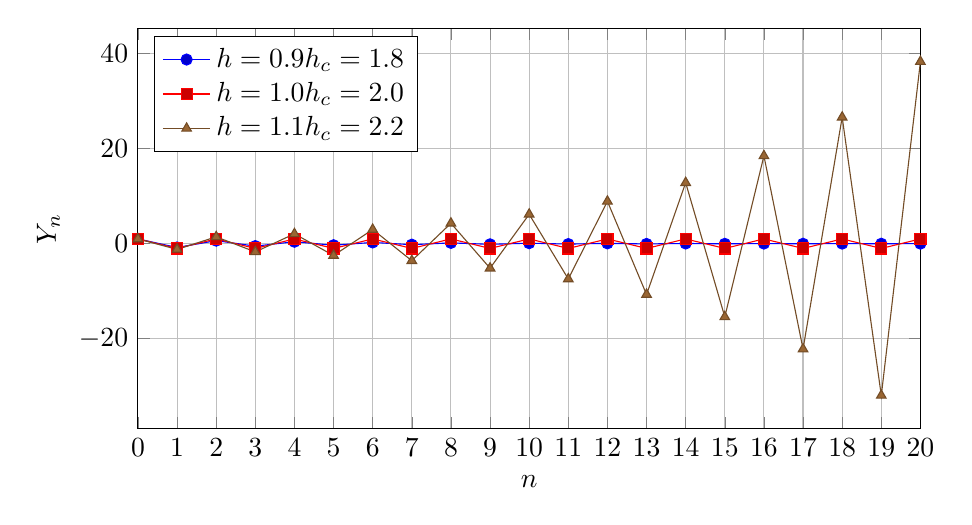
\begin{tikzpicture}
\begin{axis}[
  width=0.95\linewidth,
  height=0.55\linewidth,
  xlabel={$n$},
  ylabel={$Y_n$},
  xmin=0, xmax=20,
  xtick={0,1,2,3,4,5,6,7,8,9,10,11,12,13,14,15,16,17,18,19,20},
  grid=both,
  legend style={at={(0.02,0.98)},anchor=north west},
]
\addplot+[mark=*] coordinates {
(0,1.00000000) (1,-0.80000000) (2,0.64000000) (3,-0.51200000) (4,0.40960000)
(5,-0.32768000) (6,0.26214400) (7,-0.20971520) (8,0.16777216) (9,-0.13421773)
(10,0.10737418) (11,-0.08589935) (12,0.06871948) (13,-0.05497558) (14,0.04398047)
(15,-0.03518437) (16,0.02814750) (17,-0.02251800) (18,0.01801440) (19,-0.01441152)
(20,0.01152922)
};
\addlegendentry{$h=0.9h_c=1.8$}

\addplot+[mark=square*] coordinates {
(0,1) (1,-1) (2,1) (3,-1) (4,1) (5,-1) (6,1) (7,-1) (8,1) (9,-1)
(10,1) (11,-1) (12,1) (13,-1) (14,1) (15,-1) (16,1) (17,-1) (18,1) (19,-1) (20,1)
};
\addlegendentry{$h=1.0h_c=2.0$}

\addplot+[mark=triangle*] coordinates {
(0,1.00000000) (1,-1.20000000) (2,1.44000000) (3,-1.72800000) (4,2.07360000)
(5,-2.48832000) (6,2.98598400) (7,-3.58318080) (8,4.29981696) (9,-5.15978035)
(10,6.19173642) (11,-7.43008370) (12,8.91610044) (13,-10.69932053) (14,12.83918464)
(15,-15.40702157) (16,18.48842588) (17,-22.18611106) (18,26.62333327) (19,-31.94799993)
(20,38.33759992)
};
\addlegendentry{$h=1.1h_c=2.2$}

\end{axis}
\end{tikzpicture}
\end{center}

\section{考察（条件の妥当性）}
本課題では，厳密解$y(x)=e^{-x}$が減衰するにもかかわらず，
オイラー法では刻み幅が大きいと数値解が発散することを確認した．

実際，更新係数は$(1-h)$であり，
\[
|1-h|<1 \iff 0<h<2
\]
のときは$|Y_n|=|1-h|^n$が$n$とともに減少し（符号は交互になり得るが）発散しない．
一方で$h>2$では$|1-h|>1$となり，$|Y_n|$が指数的に増大して発散する．

したがって，オイラー法が数値的不安定となる条件を$h>h_c$と定義したとき，
この初期値問題(15)に対する限界値は
\[
\boxed{h_c=2}
\]
であり，図示結果も
\[
h=1.8\ (<2):\ \text{減衰},\qquad
h=2.0\ (=2):\ \text{振動（境界）},\qquad
h=2.2\ (>2):\ \text{発散}
\]
となって条件の妥当性が確認できた．

\end{document}
